\chapter{\noun{Use Cases} }

\begin{figure}
    \centering
    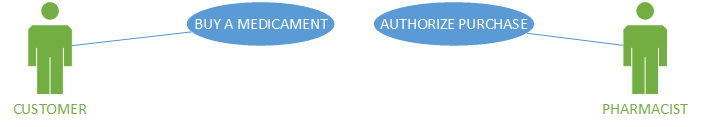
\includegraphics[width=1\textwidth]{use-case.png}
    \caption{General use case}
    \label{fig:usecase}
\end{figure} 

The way prescriptions are currently processed is vulnerable to many threats, and brings many inconveniences. The most important ones are listed below.


\begin{longtable}{|m{3cm}|m{9cm}|}
\hline 
\textbf{\noun{System's Element}} & \textbf{\noun{Use Case}}\tabularnewline
\hline 
\multirow{3}{3cm}{system} & \textbf{pharmacist\textquoteright{}s verification} - system is able
to check that pharmacist has permissions to sell the drugs\tabularnewline
\cline{2-2} 
 & \textbf{buyer\textquoteright{}s verification} - system is able to
check that the buyer\textquoteright{}s card is valid and entered PIN
number was correct\tabularnewline
\cline{2-2} 
 & \textbf{prescriptions update} - system can change the state of prescriptions
(to either \textquoteleft{}bought\textquoteright{} or \textquoteleft{}invalid\textquoteright{})
or attach additional info to them, like the fact that drug\textquoteright{}s
substitute was sold instead of prescribed one\tabularnewline
\hline 
\multirow{3}{3cm}{pharmacist} & \textbf{reading available prescriptions} - pharmacist is able to see
buyer\textquoteright{}s prescriptions\tabularnewline
\cline{2-2} 
 & \textbf{modifying the prescriptions} - pharmacist is able to update
the prescriptions (changing their state/attaching info that substitute
was sold instead)\tabularnewline
\cline{2-2} 
 & \textbf{signing the prescriptions} - pharmacist is able to sign prescription
to confirm that he\textquoteright{}s the one who sold them\tabularnewline
\hline 
\multirow{3}{3cm}{buyer} & \textbf{reading available prescriptions} - buyer is able to see/select
prescriptions that haven\textquoteright{}t yet been bought\tabularnewline
\cline{2-2} 
 & \textbf{confirming pharmacist\textquoteright{}s changes} - buyer is
obliged to confirm possible changes made to the prescriptions by the
pharmacist\tabularnewline
\cline{2-2} 
 & \textbf{signing the prescriptions} - buyer is able to sign prescription
to confirm that he got the certain medicines\tabularnewline
\hline 

\end{longtable}



